\subsection{Definitions}
\label{subsect:application-definitions}

\begin{frame}
  \frametitle{\insertsubsection}
  \begin{itemize}
    \item Drawing of ${G}$ with circular arcs \begin{itemize}
      \item Every edge ${e \in E}$ drawn as a circular arc ${\Gamma_e}$
      \item No vertices coincide
      \item No edges overlap
      \item No edge intersects any vertices other than its endpoints
    \end{itemize}
  \end{itemize}
  \centering
  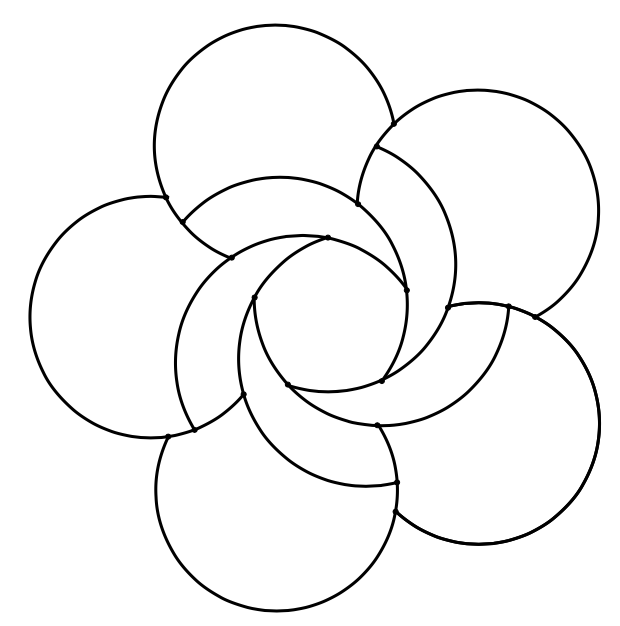
\includegraphics[height=3.5cm,natwidth=620,natheight=626]{Resources/Schulz.png}
\end{frame}

\begin{frame}
  \frametitle{\insertsubsection}
  \begin{itemize}
    \item Given a set ${\Pi = \lbrace P_1, \ldots, P_k \rbrace}$ of edge-disjoint paths \begin{itemize}
      \item ${V(\Pi) \coloneqq V(P_1) \cup \ldots \cup V(P_k)}$
      \item ${E(\Pi) \coloneqq E(P_1) \cupplus \ldots \cupplus E(P_k)}$
    \end{itemize}
    \item Drawing of ${\Pi}$ with circular arcs \begin{itemize}
      \item Drawing of ${G \coloneqq (V(\Pi), E(\Pi))}$ with circular arcs
      \item Each path ${P \in \Pi}$ is drawn as a circular arc ${\Gamma_P}$
    \end{itemize}
  \end{itemize}
  \centering
  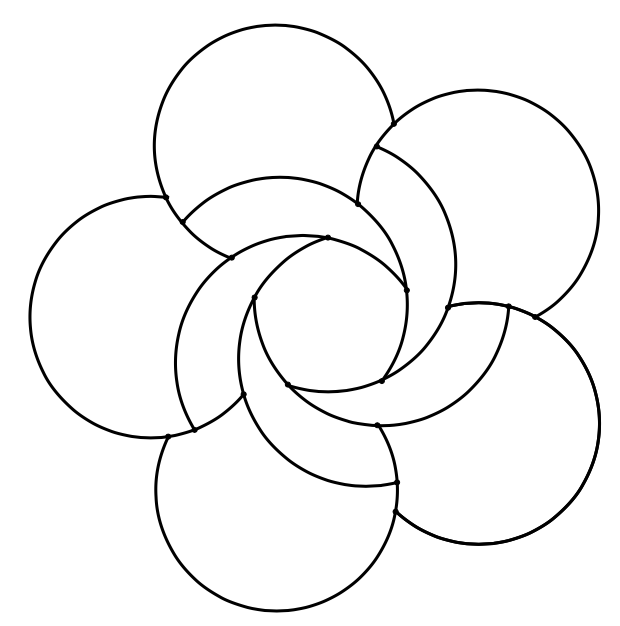
\includegraphics[height=3.5cm,natwidth=620,natheight=626]{Resources/Schulz.png}
\end{frame}
